% chapter08.tex - 狭义相对论回顾
\chapter{狭义相对论回顾 (Special Relativity Review)}
\label{chap:sr}

在进入广义相对论之前，我们有必要系统地回顾狭义相对论的核心内容。读者在前七章已经掌握了微分几何的基本工具——流形、张量、联络、曲率和测地线。现在，我们将这些工具应用于最简单但极为重要的弯曲时空的前身：\textbf{Minkowski 平直时空}。本章不仅是对狭义相对论的复习，更是用微分几何语言重新表述狭义相对论，为后续章节中从平直时空到弯曲时空的过渡做好铺垫。

\section{Minkowski 时空}

\subsection{度规与号差约定}

\begin{definition}[Minkowski 度规]
\textbf{Minkowski 时空} $(\mathbb{R}^4, \eta)$ 是配备了如下全局平直度规的四维微分流形：
\begin{equation}\label{eq:minkowski_metric}
    \dd s^2 = \eta_{\mu\nu} \dd x^\mu \dd x^\nu = -\dd t^2 + \dd x^2 + \dd y^2 + \dd z^2,
\end{equation}
其中在惯性坐标 $(x^\mu) = (t, x, y, z)$ 下（取 $c=1$ 的自然单位制），
\begin{equation}
    \eta_{\mu\nu} = \mathrm{diag}(-1, +1, +1, +1).
\end{equation}
这里采用 $(-,+,+,+)$ 号差约定。逆度规 $\eta^{\mu\nu} = \mathrm{diag}(-1, +1, +1, +1)$。
\end{definition}

\begin{note}[号差约定的选择]
在广义相对论文献中，$(-,+,+,+)$ 和 $(+,-,-,-)$ 两种号差约定都被广泛使用。本书统一使用 $(-,+,+,+)$，其优点在于：类时矢量的模方为负（$u^\mu u_\mu = -1$），空间度规为正定。这种约定使得空间部分的符号与通常的欧几里德度规一致，便于与牛顿力学对比。
\end{note}

由于度规 $\eta_{\mu\nu}$ 的所有分量均为常数，所有 Christoffel 符号恒为零：$\Gamma^\lambda_{\mu\nu} = 0$。因此，Minkowski 时空的 Riemann 曲率张量处处为零——它是\textbf{全局平坦}的伪黎曼流形。

\subsection{光锥结构}

时空间隔 $\dd s^2 = -\dd t^2 + \dd x^2 + \dd y^2 + \dd z^2$ 的符号将时空中的矢量分为三类：

\begin{definition}[矢量分类]
在 Minkowski 时空中，非零矢量 $v^\mu$ 称为：
\begin{itemize}
    \item \textbf{类时的} (timelike)：$\eta_{\mu\nu} v^\mu v^\nu < 0$（代表有质量粒子的可能世界线方向）；
    \item \textbf{类光的} (lightlike / null)：$\eta_{\mu\nu} v^\mu v^\nu = 0$（代表光子的世界线方向）；
    \item \textbf{类空的} (spacelike)：$\eta_{\mu\nu} v^\mu v^\nu > 0$（代表两个因果无关事件之间的间隔方向）。
\end{itemize}
\end{definition}

\begin{definition}[光锥]
给定时空点 $p$，所有从 $p$ 发出的类光方向构成的曲面称为 $p$ 点的\textbf{光锥} (light cone)。它分为：
\begin{itemize}
    \item \textbf{未来光锥}：$t > t_p$ 且 $\dd s^2 = 0$ 的部分；
    \item \textbf{过去光锥}：$t < t_p$ 且 $\dd s^2 = 0$ 的部分。
\end{itemize}
光锥定义了时空中事件的因果结构：只有位于光锥内部（类时分离）的事件才能与 $p$ 有因果联系。
\end{definition}

\begin{figure}[htbp]
\centering
\begin{tikzpicture}[scale=1.2]
    % Draw coordinate axes
    \draw[->,thick] (0,-3) -- (0,3) node[right] {$t$ (时间)};
    \draw[->,thick] (-3,0) -- (3,0) node[below] {$x$ (空间)};

    % Light cone (future)
    \fill[orange!20] (0,0) -- (2.5,2.5) -- (-2.5,2.5) -- cycle;
    \draw[orange,thick] (0,0) -- (2.5,2.5) node[pos=0.9,right,font=\footnotesize] {$t = x$};
    \draw[orange,thick] (0,0) -- (-2.5,2.5) node[pos=0.9,left,font=\footnotesize] {$t = -x$};

    % Light cone (past)
    \fill[blue!15] (0,0) -- (2.5,-2.5) -- (-2.5,-2.5) -- cycle;
    \draw[blue,thick] (0,0) -- (2.5,-2.5);
    \draw[blue,thick] (0,0) -- (-2.5,-2.5);

    % Labels
    \node[orange!80!black] at (1.8,2.2) {未来光锥};
    \node[blue!60!black] at (1.8,-2.2) {过去光锥};

    % A timelike worldline
    \draw[red,thick] (0,0) parabola bend (0,0) (0.5,2.5);
    \draw[red,thick,->] (0.5,2.3) -- (0.53,2.55);
    \node[red] at (1.0,1.5) {类时世界线};

    % A null worldline
    \draw[orange!80!black,thick,dashed] (0,0) -- (2.0,2.0);
    \node[orange!80!black] at (2.3,1.7) {光子};

    % Labels for regions
    \node at (2.2,0.5) {类空区域};
    \node at (-1.8,2.2) {\footnotesize 绝对未来};
    \node at (-1.8,-2.2) {\footnotesize 绝对过去};

    % Event point
    \fill (0,0) circle (0.08) node[below left] {$p$};

    % Dashed spatial line
    \draw[gray,dashed] (-2.5,1.5) -- (2.5,1.5);
    \draw[gray,dashed] (-2.5,-1.5) -- (2.5,-1.5);
\end{tikzpicture}
\caption{Minkowski 时空的光锥结构。点 $p$ 处的未来光锥（橙色）和过去光锥（蓝色）将时空划分为三个区域：绝对未来（类时 + 类光可到达）、绝对过去（类时 + 类光可影响 $p$）、以及类空区域（与 $p$ 因果无关）。红线表示有质量粒子的类时世界线，始终在光锥内部。橙色虚线表示光子的类光世界线，沿光锥表面传播。}
\label{fig:lightcone}
\end{figure}

\subsection{固有时间与世界线}

\begin{definition}[固有时间]
对于沿类时世界线 $x^\mu(\lambda)$ 运动的观测者，其\textbf{固有时间} (proper time) $\tau$ 定义为：
\begin{equation}
    \dd\tau^2 = -\dd s^2 = -\eta_{\mu\nu} \dd x^\mu \dd x^\nu = \dd t^2 - \dd\mathbf{x}^2.
\end{equation}
固有时间是观测者自身携带的理想时钟所测量的时间。仿射参数 $\tau$ 满足归一化条件：
\begin{equation}
    \eta_{\mu\nu} \frac{\dd x^\mu}{\dd\tau} \frac{\dd x^\nu}{\dd\tau} = -1.
\end{equation}
\end{definition}

\begin{example}[时间膨胀 —— 孪生子佯谬的定量计算]
考虑两个孪生子：A 留在地球（惯性系），B 以速度 $v = 0.8c$ 匀速飞向距离 $4$ 光年的恒星然后立即以相同速度返回。在 A 的坐标系中，B 去程用时 $\Delta t = 4/0.8 = 5$ 年，往返共 $10$ 年。但 B 的固有时间为：
\begin{equation}
    \Delta\tau = \sqrt{1 - v^2} \, \Delta t = \sqrt{1 - 0.64} \times 10 = 0.6 \times 10 = 6 \; \text{年}.
\end{equation}
因此，旅行归来的 B 比留守的 A 年轻了 $4$ 岁。这不是佯谬——A 的世界线是测地线（惯性运动），而 B 的世界线不是（包含加速阶段），两条世界线之间的固有时间差是客观的几何事实。
\end{example}

\section{Lorentz 变换}

\subsection{从时空间隔不变性导出 Lorentz 变换}

狭义相对论的基本假设是：物理定律在所有惯性系中具有相同的形式。在微分几何语言中，这意味着：Minkowski 时空的度规 $\eta_{\mu\nu}$ 在 Lorentz 变换下不变。

\begin{definition}[Lorentz 变换]
\textbf{Lorentz 变换} $\Lambda^\mu{}_\nu$ 是满足如下条件的线性坐标变换 $x'^\mu = \Lambda^\mu{}_\nu x^\nu$：
\begin{equation}\label{eq:lorentz_condition}
    \Lambda^\rho{}_\mu \,\eta_{\rho\sigma} \,\Lambda^\sigma{}_\nu = \eta_{\mu\nu},
\end{equation}
即 $\Lambda^T \eta \Lambda = \eta$。取行列式得 $\det\Lambda = \pm 1$。
\end{definition}

\begin{property}[Lorentz 群]
所有 Lorentz 变换构成\textbf{洛伦兹群} $\mathrm{O}(3,1)$，其李代数为 $\mathfrak{so}(3,1)$。该群有四个连通分支，由 $\det\Lambda = \pm 1$ 和 $\Lambda^0{}_0 \gtrless 0$ 的组合划分。物理上关注的\textbf{固有保时 Lorentz 群} $\mathrm{SO}^+(3,1)$ 满足 $\det\Lambda = +1$ 且 $\Lambda^0{}_0 \ge 1$（不包含空间反射和时间反演）。
\end{property}

沿 $x$ 方向的\textbf{boost}（推动）是最常用的 Lorentz 变换。设惯性系 $S'$ 相对于 $S$ 以速度 $v$ 沿 $x$ 轴运动，则：
\begin{equation}\label{eq:boost_x}
    \boxed{
    \begin{aligned}
        t' &= \gamma(t - vx), \\
        x' &= \gamma(x - vt), \\
        y' &= y, \quad z' = z,
    \end{aligned}}
\end{equation}
其中 $\gamma = 1/\sqrt{1 - v^2}$ 是 Lorentz 因子。引入\textbf{快度} (rapidity) $\phi$：
\begin{equation}
    \gamma = \cosh\phi, \qquad \gamma v = \sinh\phi, \qquad v = \tanh\phi,
\end{equation}
则 boost 变换可以写成类似于旋转的紧凑形式：
\begin{equation}\label{eq:boost_rapidity}
    \begin{pmatrix} t' \\ x' \\ y' \\ z' \end{pmatrix}
    = \begin{pmatrix}
        \cosh\phi & -\sinh\phi & 0 & 0 \\
        -\sinh\phi  & \cosh\phi  & 0 & 0 \\
        0 & 0 & 1 & 0 \\
        0 & 0 & 0 & 1
    \end{pmatrix}
    \begin{pmatrix} t \\ x \\ y \\ z \end{pmatrix}.
\end{equation}

快度参数化的最大优点在于其可加性：如果 $S''$ 相对于 $S'$ 以快度 $\phi_2$ boost，$S'$ 相对于 $S$ 以快度 $\phi_1$ boost，则 $S''$ 相对于 $S$ 的总 boost 快度为 $\phi = \phi_1 + \phi_2$。

\begin{theorem}[相对论速度加法公式]
若 $S'$ 相对于 $S$ 以速度 $v$ 沿 $x$ 轴运动，在 $S'$ 中一粒子以速度 $u'$ 沿 $x$ 轴运动，则该粒子在 $S$ 中的速度为：
\begin{equation}\label{eq:velocity_addition}
    u = \frac{u' + v}{1 + u'v}.
\end{equation}
用快度表示即为 $\phi_u = \phi_{u'} + \phi_v$，对应快度的简单相加。
\end{theorem}

\begin{example}[速度加法与光速不变]
若 $u' = 1$（光速），则 $u = \frac{1 + v}{1 + v} = 1$——无论 $v$ 多大，光速在任意惯性系中始终保持不变。这是 Lorentz 变换的直接推论。
\end{example}

\subsection{Lorentz 变换的生成元}

无穷小 Lorentz 变换可写为：
\begin{equation}
    \Lambda^\mu{}_\nu = \delta^\mu{}_\nu + \omega^\mu{}_\nu, \qquad |\omega^\mu{}_\nu| \ll 1.
\end{equation}
由 $\Lambda^T\eta\Lambda = \eta$ 得 $\omega_{\mu\nu} = -\omega_{\nu\mu}$（其中 $\omega_{\mu\nu} = \eta_{\mu\rho}\omega^\rho{}_\nu$）。反对称矩阵 $\omega_{\mu\nu}$ 有 $6$ 个独立参数：$3$ 个对应空间旋转（$\omega_{ij}$），$3$ 个对应 boost（$\omega_{0i}$）。

\begin{figure}[htbp]
\centering
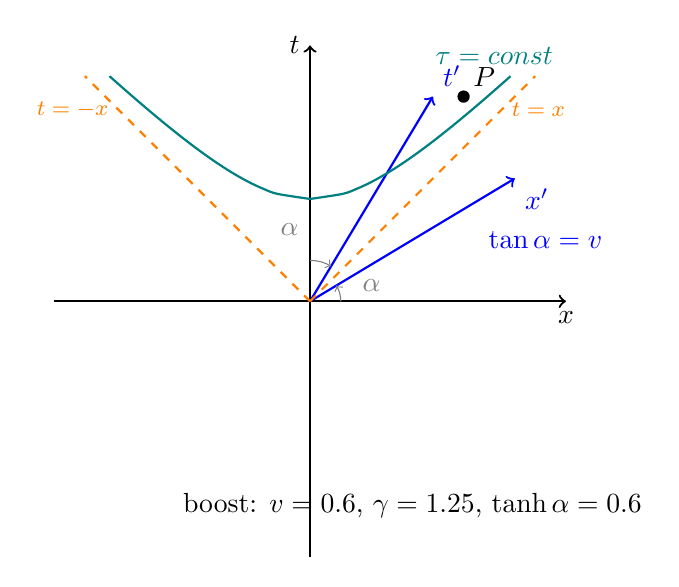
\begin{tikzpicture}[scale=1.3]
    % Original axes (t, x)
    \draw[->,thick] (0,-2.5) -- (0,2.5) node[left] {$t$};
    \draw[->,thick] (-2.5,0) -- (2.5,0) node[below] {$x$};

    % Boosted axes (t', x') - rotated towards light cone
    % t' axis: x = v t, i.e., line with slope 1/v in (t,x) plane
    % For v = 0.6, slope = 1/0.6 ≈ 1.67, angle ≈ 59° from t-axis
    % In (x,t) coordinates on paper: t is vertical, x is horizontal
    % t' axis: t = x/v, so for v=0.6, t = 1.67x
    \draw[->,blue,thick] (0,0) -- (1.2,2.0) node[above right] {$t'$};
    % x' axis: t = vx, so for v=0.6, t = 0.6x
    \draw[->,blue,thick] (0,0) -- (2.0,1.2) node[below right] {$x'$};

    % Light cone lines
    \draw[orange,thick,dashed] (0,0) -- (2.2,2.2) node[pos=0.85,right,font=\footnotesize] {$t=x$};
    \draw[orange,thick,dashed] (0,0) -- (-2.2,2.2) node[pos=0.85,left,font=\footnotesize] {$t=-x$};

    % Angle annotations
    \draw[->,gray] (0.3,0) arc (0:31:0.3);
    \node[gray] at (0.6,0.15) {$\alpha$};
    \draw[->,gray] (0,0.4) arc (90:59:0.4);
    \node[gray] at (-0.2,0.7) {$\alpha$};

    % v=c scaling note
    \node at (1.0, -2.0) {boost: $v = 0.6$, $\gamma = 1.25$, $\tanh\alpha = 0.6$};
    \node[blue] at (2.3, 0.6) {$\tan\alpha = v$};

    % Hyperbola of constant proper time
    \draw[teal,thick,domain=1.0:2.2,smooth,variable=\t] plot ({sqrt(\t*\t-1)},\t);
    \draw[teal,thick,domain=1.0:2.2,smooth,variable=\t] plot ({-sqrt(\t*\t-1)},\t);
    \node[teal] at (1.8, 2.4) {$\tau = \text{const}$};

    % Point P with coordinates in both frames
    \fill (1.5, 2.0) circle (0.06) node[above right] {$P$};
\end{tikzpicture}
\caption{Lorentz boost 的 Minkowski 时空图。黑色轴为原惯性系 $(t, x)$，蓝色轴为以速度 $v = 0.6$ 相对运动的惯性系 $(t', x')$。$t'$ 轴与 $x'$ 轴关于光锥（橙色虚线）对称——它们之间夹角为 $2\alpha$，其中 $\tanh\alpha = v$。青色曲线代表固有时间 $\tau$ 为常数的双曲线——所有惯性系中具有相同固有时间的事件位于同一条双曲线上。}
\label{fig:lorentz_boost}
\end{figure}

\section{四维矢量与张量}

狭义相对论中的物理量自然组织为 Minkowski 时空上的四维张量。三维空间中的矢量（如速度、动量）只是四维对应量的空间分量——它们在不同惯性系下混合。

\subsection{四速度与四动量}

\begin{definition}[四速度]
粒子的\textbf{四速度} (4-velocity) 定义为世界线对固有时间的导数：
\begin{equation}
    u^\mu = \frac{\dd x^\mu}{\dd\tau}.
\end{equation}
由 $\dd\tau^2 = -\eta_{\mu\nu}\dd x^\mu\dd x^\nu$，四速度自动满足归一化条件：
\begin{equation}\label{eq:u_normalization}
    \eta_{\mu\nu} u^\mu u^\nu = -1.
\end{equation}
\end{definition}

在惯性系中，粒子的三维速度为 $\mathbf{v} = \dd\mathbf{x}/\dd t$，则：
\begin{equation}\label{eq:4velocity_components}
    \boxed{u^\mu = \gamma\,(1, \mathbf{v})}, \qquad u_\mu = \eta_{\mu\nu} u^\nu = \gamma\,(-1, \mathbf{v}),
\end{equation}
其中 $\gamma = 1/\sqrt{1 - v^2}$。可以验证 $u^\mu u_\mu = \gamma^2(-1 + v^2) = -1$。

\begin{definition}[四动量]
质量为 $m$ 的粒子的\textbf{四动量} (4-momentum) 为：
\begin{equation}
    p^\mu = m u^\mu = (E, \mathbf{p}),
\end{equation}
其中 $E = \gamma m$ 是相对论能量，$\mathbf{p} = \gamma m \mathbf{v}$ 是相对论动量。
\end{definition}

\begin{property}[质壳条件]
四动量的模方给出著名的 Einstein 能量-动量关系：
\begin{equation}\label{eq:mass_shell}
    \boxed{p^\mu p_\mu = -E^2 + \mathbf{p}^2 = -m^2}.
\end{equation}
这是一个 Lorentz 不变量——在所有惯性系中，$E^2 - \mathbf{p}^2 = m^2$ 恒成立。此关系定义了动量空间中的\textbf{质壳} (mass shell)。
\end{property}

\begin{example}[四速度分量的计算]
考虑一个以速度 $v = 0.6$ 沿 $x$ 轴运动的粒子。计算其四速度分量。
\[
\gamma = \frac{1}{\sqrt{1 - 0.36}} = \frac{1}{0.8} = 1.25.
\]
因此：
\[
u^\mu = \gamma(1, v, 0, 0) = (1.25,\, 0.75,\, 0,\, 0).
\]
验证归一化：$u^\mu u_\mu = -(1.25)^2 + (0.75)^2 = -1.5625 + 0.5625 = -1$。\hfill $\checkmark$

四动量为 $p^\mu = m u^\mu$。在 $v \ll 1$ 的低速极限下：
\[
E = \gamma m = \frac{m}{\sqrt{1 - v^2}} \approx m\Bigl(1 + \frac{v^2}{2}\Bigr) = m + \frac{1}{2}mv^2,
\]
即静止能量 $m$ 加上牛顿动能 $\frac{1}{2}mv^2$。这正是 Einstein 质能关系的根源。
\end{example}

\subsection{四加速度与四力}

\begin{definition}[四加速度]
\textbf{四加速度} (4-acceleration) 是四速度对固有时间的协变导数。在 Minkowski 时空（$\Gamma^\lambda_{\mu\nu} = 0$）中，即普通导数：
\begin{equation}
    a^\mu = \frac{\dd u^\mu}{\dd\tau} = \frac{\dd^2 x^\mu}{\dd\tau^2}.
\end{equation}
由 $u^\mu u_\mu = -1$ 求导得 $a^\mu u_\mu = 0$——四加速度总是与四速度正交。
\end{definition}

\begin{definition}[四力]
\textbf{四力} (4-force) 或 Minkowski 力定义为：
\begin{equation}
    f^\mu = \frac{\dd p^\mu}{\dd\tau} = m a^\mu.
\end{equation}
其空间分量与三维力 $\mathbf{F} = \dd\mathbf{p}/\dd t$ 的关系为 $f^i = \gamma F^i$，时间分量 $f^0 = \gamma\,\mathbf{F}\cdot\mathbf{v}$（即功率）。
\end{definition}

\section{能量--动量张量}

在狭义相对论中，连续介质（流体、场）的能量、动量和应力分布被统一编码在\textbf{能量--动量张量} $T^{\mu\nu}$（也称应力--能量张量）中。

\subsection{完美流体}

\begin{definition}[完美流体的能量--动量张量]
\textbf{完美流体} (perfect fluid) 是理想化的连续介质，在其静止系中无黏滞性和热传导。其能量--动量张量为：
\begin{equation}\label{eq:perfect_fluid}
    \boxed{T^{\mu\nu} = (\rho + p)\,u^\mu u^\nu + p\,\eta^{\mu\nu}},
\end{equation}
其中：
\begin{itemize}
    \item $\rho$ —— 随动系中的\textbf{能量密度} (energy density)；
    \item $p$ —— 随动系中的\textbf{压强} (pressure)；
    \item $u^\mu$ —— 流体元的四速度场。
\end{itemize}
在流体的静止系中（$u^\mu = (1, \mathbf{0})$），能量--动量张量取对角形式：
\begin{equation}
    T^{\mu\nu} = \begin{pmatrix}
        \rho & 0 & 0 & 0 \\
        0 & p & 0 & 0 \\
        0 & 0 & p & 0 \\
        0 & 0 & 0 & p
    \end{pmatrix}.
\end{equation}
\end{definition}

\begin{note}[$T^{\mu\nu}$ 各分量的物理解释]
在一般惯性系中，$T^{\mu\nu}$ 的分量具有清晰的物理含义：
\begin{itemize}
    \item $T^{00}$：能量密度（单位体积内的能量）；
    \item $T^{0i} = T^{i0}$：动量密度 / 能量流密度（第 $i$ 方向单位面积、单位时间内流过的能量）；
    \item $T^{ij}$：应力张量——第 $i$ 方向单位面积上作用的第 $j$ 方向力。对角元 $T^{ii}$（无求和）是正应力（压强），非对角元 $T^{ij}$ ($i\neq j$) 是切应力。
\end{itemize}
\end{note}

\subsection{能量--动量守恒}

在平直时空中，能量--动量守恒表现为能量--动量张量的四维散度为零：
\begin{equation}\label{eq:conservation}
    \boxed{\partial_\mu T^{\mu\nu} = 0}.
\end{equation}
这实际上包含了四个守恒方程：
\begin{itemize}
    \item $\nu = 0$：能量守恒 $\partial_t T^{00} + \partial_i T^{i0} = 0$；
    \item $\nu = i$：动量守恒 $\partial_t T^{0i} + \partial_j T^{ji} = 0$。
\end{itemize}

对于完美流体，代入 (\ref{eq:perfect_fluid}) 后，守恒方程 $\partial_\mu T^{\mu\nu} = 0$ 投影为：
\begin{equation}
    u^\nu \partial_\nu \rho + (\rho + p)\partial_\nu u^\nu = 0 \quad\text{(能量守恒，沿流线)},
\end{equation}
\begin{equation}
    (\rho + p) u^\nu \partial_\nu u^\mu = -(\eta^{\mu\nu} + u^\mu u^\nu)\,\partial_\nu p \quad\text{(相对论 Euler 方程)}.
\end{equation}

\subsection{尘埃与辐射}

\begin{definition}[尘埃]
\textbf{尘埃} (dust) 是压强可以忽略的完美流体（$p=0$）：
\begin{equation}
    T^{\mu\nu}_{\text{dust}} = \rho\, u^\mu u^\nu.
\end{equation}
尘埃描述无相互作用的粒子集合（如宇宙学中的冷暗物质）。尘埃的每个流体元沿测地线运动：
\begin{equation}
    u^\nu \partial_\nu (\rho u^\mu) = 0.
\end{equation}
\end{definition}

\begin{definition}[辐射]
\textbf{辐射} (radiation) 或极端相对论流体对应无质量粒子气体，其状态方程为 $p = \rho/3$。能量--动量张量为：
\begin{equation}
    T^{\mu\nu}_{\text{rad}} = \frac{4}{3}\rho\,u^\mu u^\nu + \frac{1}{3}\rho\,\eta^{\mu\nu},
\end{equation}
且满足无迹条件 $T^\mu{}_\mu = 0$。这是电磁辐射和极端相对论粒子气体的基本特征。
\end{definition}

\section{Maxwell 方程的协变形式}

Maxwell 的电动力学是狭义相对论的最早成功应用。本节用四维张量语言重新表述电磁理论，展示其内蕴的 Lorentz 协变性。

\subsection{四维势与场强张量}

\begin{definition}[电磁四维势]
\textbf{电磁四维势} (electromagnetic 4-potential) $A_\mu$ 将标量势 $\phi$ 和矢量势 $\mathbf{A}$ 统一为：
\begin{equation}
    A_\mu = (-\phi, \mathbf{A}), \qquad A^\mu = \eta^{\mu\nu}A_\nu = (\phi, \mathbf{A}).
\end{equation}
\end{definition}

\begin{definition}[电磁场强张量]
\textbf{电磁场强张量} (field strength tensor) $F_{\mu\nu}$ 定义为四维势的外导数：
\begin{equation}\label{eq:F_definition}
    \boxed{F_{\mu\nu} = \partial_\mu A_\nu - \partial_\nu A_\mu}.
\end{equation}
$F_{\mu\nu}$ 是反对称的 $(0,2)$ 型张量：$F_{\mu\nu} = -F_{\nu\mu}$。其分量与电场 $\mathbf{E}$ 和磁场 $\mathbf{B}$ 的关系为：
\begin{equation}\label{eq:F_components}
    F_{\mu\nu} = \begin{pmatrix}
        0 & -E_x & -E_y & -E_z \\
        E_x & 0 & B_z & -B_y \\
        E_y & -B_z & 0 & B_x \\
        E_z & B_y & -B_x & 0
    \end{pmatrix}, \qquad
    F^{\mu\nu} = \begin{pmatrix}
        0 & E_x & E_y & E_z \\
        -E_x & 0 & B_z & -B_y \\
        -E_y & -B_z & 0 & B_x \\
        -E_z & B_y & -B_x & 0
    \end{pmatrix}.
\end{equation}
\end{definition}

\begin{note}[规范不变性]
四维势 $A_\mu$ 不是唯一的。规范变换 $A_\mu \to A_\mu + \partial_\mu \Lambda$（对任意标量函数 $\Lambda$）不改变场强张量：$F_{\mu\nu} \to F_{\mu\nu}$。这是 $U(1)$ 规范对称性的表现。
\end{note}

\subsection{Maxwell 方程的协变形式}

在四维张量语言中，四个 Maxwell 方程被紧凑地表述为两个张量方程。

\begin{theorem}[Maxwell 方程 —— 协变形式]
有源 Maxwell 方程（Gauss 定律和 Ampère 定律）统一为：
\begin{equation}\label{eq:maxwell_source}
    \boxed{\partial_\mu F^{\mu\nu} = J^\nu},
\end{equation}
其中 $J^\nu = (\rho_e, \mathbf{J})$ 是\textbf{四维电流密度}（$\rho_e$ 为电荷密度，$\mathbf{J}$ 为三维电流密度）。此处已取单位制使 $\mu_0 = \varepsilon_0 = 1$。

无源 Maxwell 方程（Gauss 磁定律和 Faraday 定律）统一为\textbf{Bianchi 恒等式}：
\begin{equation}\label{eq:maxwell_bianchi}
    \boxed{\partial_{[\mu} F_{\nu\rho]} = 0},
\end{equation}
即 $\partial_\mu F_{\nu\rho} + \partial_\nu F_{\rho\mu} + \partial_\rho F_{\mu\nu} = 0$。这是场强张量由四维势定义的自动推论（等价于 $\dd F = 0$，其中 $F = \frac{1}{2}F_{\mu\nu}\dd x^\mu \wedge \dd x^\nu$）。
\end{theorem}

\begin{example}[验证 Maxwell 方程的 Lorentz 协变性]
我们显式验证方程 (\ref{eq:maxwell_source}) 和 (\ref{eq:maxwell_bianchi}) 在 Lorentz 变换下保持形式不变。

设 Lorentz 变换 $x'^\mu = \Lambda^\mu{}_\nu x^\nu$。张量分量的变换规则为：
\[
F'^{\mu\nu} = \Lambda^\mu{}_\rho \Lambda^\nu{}_\sigma F^{\rho\sigma}, \qquad
J'^\nu = \Lambda^\nu{}_\rho J^\rho.
\]
偏导数的变换为 $\partial'_\mu = (\Lambda^{-1})^\nu{}_\mu \partial_\nu$。在 Lorentz 变换下：
\[
\partial'_\mu F'^{\mu\nu} = (\Lambda^{-1})^\alpha{}_\mu \partial_\alpha (\Lambda^\mu{}_\rho \Lambda^\nu{}_\sigma F^{\rho\sigma})
= \Lambda^\nu{}_\sigma (\Lambda^{-1})^\alpha{}_\mu \Lambda^\mu{}_\rho \,\partial_\alpha F^{\rho\sigma}
= \Lambda^\nu{}_\sigma \,\partial_\rho F^{\rho\sigma} = \Lambda^\nu{}_\sigma J^\sigma = J'^\nu.
\]
因此 $\partial_\mu F^{\mu\nu} = J^\nu$ 在 Lorentz 变换下保持形式不变——它是张量方程。同样的推理适用于 $\partial_{[\mu}F_{\nu\rho]} = 0$。\hfill $\square$
\end{example}

\subsection{Lorentz 力的协变形式}

\begin{theorem}[Lorentz 力 —— 协变形式]
电荷为 $q$ 的带电粒子在电磁场中受到的\textbf{Lorentz 四力}为：
\begin{equation}\label{eq:lorentz_force}
    \boxed{f^\mu = q\,F^{\mu\nu} u_\nu},
\end{equation}
其中 $u^\nu$ 是粒子的四速度。此方程同时包含了三维 Lorentz 力 $\mathbf{F} = q(\mathbf{E} + \mathbf{v}\times\mathbf{B})$ 和功率方程 $\dd E/\dd t = q\mathbf{E}\cdot\mathbf{v}$。
\end{theorem}

\begin{proof}[Lorentz 力的分量展开]
展开 $f^\mu = q F^{\mu\nu}u_\nu$。对于 $\mu = i$（空间分量）：
\[
f^i = q(F^{i0}u_0 + F^{ij}u_j) = q\bigl(E^i \cdot (-\gamma) + \varepsilon^{ijk}B_k \cdot (\gamma v^j)\bigr)
= q\gamma\,(E^i + (\mathbf{v}\times\mathbf{B})^i).
\]
由于 $f^i = \gamma F^i$，得 $F^i = q(E^i + (\mathbf{v}\times\mathbf{B})^i)$——即三维 Lorentz 力。

对于 $\mu = 0$（时间分量）：
\[
f^0 = q F^{0j}u_j = q E^j \cdot (\gamma v^j) = q\gamma\,\mathbf{E}\cdot\mathbf{v}.
\]
由于 $f^0 = \gamma\,\dd E/\dd t$，得 $\dd E/\dd t = q\mathbf{E}\cdot\mathbf{v}$——即电磁场对带电粒子做功的功率。
\end{proof}

\subsection{能量--动量张量的电磁对应物}

电磁场本身携带着能量和动量。电磁场的能量--动量张量为：
\begin{equation}\label{eq:em_stress_energy}
    T^{\mu\nu}_{\text{EM}} = F^{\mu\rho} F^\nu{}_\rho - \frac{1}{4}\eta^{\mu\nu} F_{\rho\sigma}F^{\rho\sigma}.
\end{equation}
其分量与电磁场的能量密度 $u = \frac{1}{2}(\mathbf{E}^2 + \mathbf{B}^2)$、Poynting 矢量 $\mathbf{S} = \mathbf{E}\times\mathbf{B}$ 以及 Maxwell 应力张量的关系为：
\begin{equation}
    T^{00}_{\text{EM}} = \frac{1}{2}(\mathbf{E}^2 + \mathbf{B}^2), \quad
    T^{0i}_{\text{EM}} = (\mathbf{E}\times\mathbf{B})^i, \quad
    T^{ij}_{\text{EM}} = -E^i E^j - B^i B^j + \frac{1}{2}\delta^{ij}(\mathbf{E}^2 + \mathbf{B}^2).
\end{equation}
可以验证 $\partial_\mu T^{\mu\nu}_{\text{EM}} = -F^{\nu\rho}J_\rho$——电磁场的能量--动量不是独立守恒的，而是与带电物质交换能量和动量。

\subsection{不变量与对偶}

\begin{example}[电磁场的不变量：$\mathbf{E}^2 - \mathbf{B}^2$ 和 $\mathbf{E}\cdot\mathbf{B}$]
电磁场有两个独立的 Lorentz 不变量：
\[
F_{\mu\nu}F^{\mu\nu} = 2(\mathbf{B}^2 - \mathbf{E}^2), \qquad
\tilde{F}_{\mu\nu}F^{\mu\nu} = -4\,\mathbf{E}\cdot\mathbf{B},
\]
其中 $\tilde{F}_{\mu\nu} = \frac{1}{2}\varepsilon_{\mu\nu\rho\sigma}F^{\rho\sigma}$ 是 Hodge 对偶场强（$\varepsilon_{0123} = 1$）。

这两个不变量的物理意义：
\begin{itemize}
    \item 若 $\mathbf{B}^2 > \mathbf{E}^2$（磁场主导），则存在惯性系使得电场为零；
    \item 若 $\mathbf{E}^2 > \mathbf{B}^2$（电场主导），则存在惯性系使得磁场为零；
    \item 若 $\mathbf{E}\cdot\mathbf{B} \neq 0$，则电磁场具有手性（如在电磁波中 $\mathbf{E}\cdot\mathbf{B} = 0$，即电场与磁场正交）；
    \item 平面电磁波满足 $F_{\mu\nu}F^{\mu\nu} = 0$ 和 $\tilde{F}_{\mu\nu}F^{\mu\nu} = 0$——两个不变量同时为零。
\end{itemize}
\end{example}

\section{从狭义相对论到广义相对论}

经过以上各节的回顾，我们现在处于一个关键的分水岭：我们已经在 Minkowski 平直时空中建立了完整的相对论物理学框架。但狭义相对论有一个根本性的局限——它无法容纳引力。

\subsection{狭义相对论的局限}

\begin{remark}[狭义相对论为何不能描述引力]
狭义相对论在以下方面与引力不相容：
\begin{enumerate}
    \item \textbf{引力的普适性与惯性系的优先地位}：狭义相对论赋予惯性系以特殊地位，但引力的普适性（所有物体同样下落）表明，引力场中的\textbf{自由下落参考系}才是真正的\"惯性系\"——而这正是非惯性系。
    \item \textbf{引力的潮汐效应}：两个相邻自由下落粒子之间的相对加速度（潮汐力）无法在平直时空的框架内描述，因为零曲率意味着相邻测地线永远平行——但实际引力场中它们会汇聚或发散。
    \item \textbf{光在引力场中的偏折}：狭义相对论预言光沿直线传播（类光测地线在平直时空中是直线），但实际观测（1919年日食观测）证实了星光经过太阳附近时发生偏折。
    \item \textbf{牛顿引力的瞬时传播}：牛顿引力是超距作用，违反狭义相对论的光速极限。任何相对论性的引力理论必须以有限速度传播。
    \item \textbf{等效原理}：惯性质量与引力质量的精确相等（Eötvös 实验精度已达 $10^{-15}$）是一个深刻的谜团，暗示引力与惯性之间存在本质联系——这种联系在平直时空的框架内无法自然解释。
\end{enumerate}
\end{remark}

\subsection{Einstein 的洞察：引力 = 时空弯曲}

\begin{note}[从平直时空到弯曲时空的关键跃迁]
Einstein 的洞见可以概括为三个递进的层次：
\begin{enumerate}
    \item \textbf{等效原理}：在局部范围内，引力和加速度不可区分。这意味着自由下落参考系中的物理定律与狭义相对论中的形式相同——在时空的每个点上，存在一个局部惯性系，其中度规取 Minkowski 形式 $\eta_{\mu\nu}$ 且 Christoffel 符号为零。
    \item \textbf{引力的几何化}：既然局部惯性系因时空点而异（不同点的自由下落参考系彼此有相对加速度），唯一的可能是时空本身是弯曲的。引力不再是一种\"力\"，而是时空弯曲的表现。
    \item \textbf{度规作为引力势}：Minkowski 度规 $\eta_{\mu\nu}$ 被推广为一般弯曲时空中的动力学度规场 $g_{\mu\nu}(x)$。在局部惯性系中 $g_{\mu\nu}$ 约化为 $\eta_{\mu\nu}$，但 $g_{\mu\nu}$ 的二阶导数（曲率）体现了真实的引力场——潮汐力。这与牛顿引力势 $\Phi$ 的角色完全平行：$\Phi$ 本身可以通过坐标变换消除（等效原理），但其二阶导数是物理的（潮汐张量）。
\end{enumerate}
\end{note}

\begin{theorem}[最小耦合原理 —— 预览]
从狭义相对论过渡到广义相对论的\"处方\"是\textbf{最小耦合原理} (minimal coupling principle)：
\begin{equation}\label{eq:minimal_coupling}
    \boxed{\eta_{\mu\nu} \;\longrightarrow\; g_{\mu\nu}(x), \qquad \partial_\mu \;\longrightarrow\; \nabla_\mu}.
\end{equation}
即，将平直时空度规替换为弯曲时空度规，将普通导数替换为协变导数。在此规则下，狭义相对论的所有物理定律被\"提升\"为广义相对论中弯曲时空的物理定律。

例如，自由粒子从 $m\,\dd^2 x^\mu / \dd\tau^2 = 0$（平直时空）提升为测地线方程 $\dd^2 x^\mu/\dd\tau^2 + \Gamma^\mu_{\nu\rho} \dot x^\nu \dot x^\rho = 0$（弯曲时空）；能量--动量守恒从 $\partial_\mu T^{\mu\nu} = 0$ 提升为 $\nabla_\mu T^{\mu\nu} = 0$。
\end{theorem}

\begin{note}[本章总结与展望]
本章用微分几何的语言系统回顾了狭义相对论的核心内容：
\begin{itemize}
    \item Minkowski 时空是全局平坦的伪黎曼流形 $(\mathbb{R}^4, \eta)$，光锥定义了因果结构；
    \item Lorentz 变换是保持 $\eta_{\mu\nu}$ 不变的线性变换，构成群 $\mathrm{SO}^+(3,1)$；
    \item 物理量被统一为四维张量——四速度、四动量、能量--动量张量；
    \item Maxwell 方程以 $F_{\mu\nu}$ 的简洁形式展现了其内蕴的 Lorentz 协变性；
    \item 狭义相对论的根本局限在于无法容纳引力，而 Einstein 的解决方案是：\textbf{放弃平直时空，拥抱弯曲时空}。
\end{itemize}

从下一章开始，我们将进入广义相对论的核心：等效原理、广义协变性、爱因斯坦场方程，以及它们如何将\"引力 = 时空弯曲\"这一深刻思想转化为精确的数学理论。
\end{note}

%=============================================================================
% 习题
%=============================================================================

\section*{本章习题}

\begin{enumerate}
    \item 验证快度参数化的 boost 矩阵 (\ref{eq:boost_rapidity}) 满足 Lorentz 条件 $\Lambda^T\eta\Lambda = \eta$。
    \item 从 $E^2 - \mathbf{p}^2 = m^2$ 出发，推导相对论粒子的速度-动量关系 $\mathbf{v} = \mathbf{p}/E$。
    \item 验证电磁场强张量 (\ref{eq:F_definition}) 在规范变换 $A_\mu \to A_\mu + \partial_\mu\Lambda$ 下不变。
    \item 从 $\partial^\mu T^{\text{EM}}_{\mu\nu} = -F_{\nu\rho}J^\rho$ 出发，推导 Poynting 定理（电磁能量守恒）。
    \item 证明平面电磁波满足 $F_{\mu\nu}F^{\mu\nu} = 0$ 和 $\tilde{F}_{\mu\nu}F^{\mu\nu} = 0$。
    \item 利用 Lorentz 变换，证明在一个惯性系中的纯电场，在另一个以速度 $\mathbf{v}$ 相对运动的惯性系中会产生磁场。
\end{enumerate}
